\documentclass[10pt,twoside,lineno]{gsajnl}
\articletype{inv} % article type

\usepackage[dvipsnames]{xcolor}
\usepackage{amsmath}
\usepackage{amssymb}
\usepackage{natbib}
\usepackage[linesnumbered,ruled,vlined,algo2e]{algorithm2e}
\usepackage{tikz}
\usetikzlibrary{arrows, snakes,backgrounds}
\tikzstyle{place}=[circle,draw=black,thick, inner sep=0pt, minimum size = 5mm]
\usepackage{hyperref}
\hypersetup{
	pagebackref=true,
	colorlinks = true,
	allcolors = OliveGreen}

\SetKwInput{input}{Input}
\SetKwInput{output}{Output}


\newcommand{\E}{\mathbb{E}}
\renewcommand{\P}{\mathbb{P}}
\newcommand{\R}{\mathbb{R}}
\newcommand{\T}{\mathbb{T}}
\newcommand{\ind}{\mathbf{1}}
\newcommand{\tn}{\textnormal}
\newcommand{\ov}{\overline}
\newcommand{\tskit}{\texttt{tskit}}
\newcommand{\tsinfer}{\texttt{tsinfer}}
\newcommand{\msprime}{\texttt{msprime}}
\newcommand{\argmax}{\operatorname{argmax}}
\newcommand{\dis}{\operatorname{dis}}
\newcommand{\similarity}{\operatorname{sim}}
\newcommand{\comment}[1]{{\color{violet} \it #1}}

\newcommand{\algorithmref}[2][]{%
	\hyperref[{#2}]{%
		Algorithm~\ref*{#2}%
		\ifx\\#1\\%
		\else
		\,#1%
		\fi
	}%
}

\newcommand*{\figref}[2][]{%
	\hyperref[{#2}]{%
		Figure~\ref*{#2}%
		\ifx\\#1\\%
		\else
		\,#1%
		\fi
	}%
}

\newcommand*{\tabref}[2][]{%
	\hyperref[{#2}]{%
		Table~\ref*{#2}%
		\ifx\\#1\\%
		\else
		\,#1%
		\fi
	}%
}
\newcommand*{\eqnref}[2][]{%
	\hyperref[{#2}]{%
		Equation~\ref*{#2}%
		\ifx\\#1\\%
		\else
		\,#1%
		\fi
	}%
}


\title{
    A forest is more than its trees:
    haplotypes and inferred ARGs
}

% Information in recombination junctions can both compress and improve inferred tree sequences
% Non-coalescing regions of dark matter in ARGs
% Can we find them? Are they useful in inference, dating? 
% Look, we can find them and they seem at least useful for compression.
% Also, here's a way of measuring agreement that takes this sort of thing into account,
%  which extends R-F to measure haplotypes


\author[$\dagger$]{Halley Fritze}
\author[$\ast$]{Nathaniel Pope}
\author[$\ddagger$]{Jerome Kelleher}
\author[$\ast$,$\dagger$,S]{Peter Ralph}

\affil[$\ast$]{Institute of Evolution and Ecology and Department of Biology, University of Oregon, Eugene, Oregon}
\affil[$\dagger$]{Department of Mathematics, University of Oregon, Eugene, Oregon}
\affil[$\ddagger$]{Big Data Institute, Li Ka Shing Centre for Health Information and Discovery, University of Oxford}
\affil[$\S$]{Department of Data Science, University of Oregon, Eugene, Oregon}


\keywords{genealogy, tree sequence, haplotypes}

\runningtitle{Haplotypes in ARGs}
\runningauthor{Fritze \textit{et al.}}

%%%%%%%%%%
\begin{abstract}
    Foreshadowing haplotype-based methods of the genomics era,
    it is an old observation that the ``junction'' between two distinct haplotypes
    produced by recombination is inherited as a Mendelian marker.
    In this paper, we describe how this recombination-mediated information
    can in many cases be recovered from inference based solely on polymorphic markers.
    % NSP-22NOV: "unary node" and "ARG" are not defined so I tried to provide better context here
    In a genealogical context, this information reflects the persistence
    of ancestral haplotypes across marginal genealogical trees where they
    are not coalescence events.
    We show how these non-coalescing haplotypes (``unary nodes'') may be
    inserted into the ancestral recombination graph (ARG), a compact
    but information-rich data structure describing the genealogical
    relationships among recombinant sequences.
    The resulting inferred ARGs are smaller, faster to compute with,
    and contain substantially more information % NSP-22NOV: "substantially more information" in what regard?
    than inferred ARGs without unary nodes.
    We provide efficient algorithms to infer unary nodes within existing ARGs,
    new metrics of agreement and disagreement between inferred ARGs,
    and explore some consequences of unary nodes for ARGs inferred from real data.
\end{abstract}

\begin{document}

\maketitle
\thispagestyle{firststyle}
\marginmark
\firstpagefootnote

\correspondingauthoraffiliation{1}{Corresponding author: {plr@uoregon.edu}}
\vspace{-33pt}% Only used for adjusting extra space in the left column of the first page


%%% OUTLINE
% Intro: haplotypes, unary bits of non-coalescing nodes, ARGS, etcetera
%    explain what tsinfer does to create unary regions
%    statement of problem
%    Yan: are breakpoints in true->simplify->extend the same as in original?
%   Fig 1: conceptual figure
%    Also IBD gets screwed up
% 
% Methods:
%   edge extend algorithm
%   discrepancy funciton algorithm
%   Fig 2: Conceptual figure for discrepancy
% 
% Results:
%   Fig 3:
%     (a) reduction in number of edges and (b) speed change
%
%   Fig 4:
%     Histograms of (a) total span added, (b) percent incorrect
%
%   Fig 5 and maybe 6: how it interacts with tsinfer
%     (a) summarize total matching and unmatching span (or maybe percent matching?)
%           across reps
%     (b) discrepancy per node against depth or time or number of subtended samples
%        describe percent span matched against true span or depth or something
%
%   Fig 7(?): compare IBD stats before/after
% 
% Supp:
%   S1: runtime
%%%


% Name ideas:
% 
% extend edges
% bundle edges
% inflate edges
% bundle lines of descent
% longer ancestral haplotypes
% inflated ancestors
% compress paths
% optimizing edge tables
% reduce number of ancestors
% reduce ancestral paths


%%%% COLOR SCHEME FOR FIGURES %%%%
% colors = {'blue': 'rgb(46,37,133)',
%	'red': 'rgb(194,106,119)',
%	'lgreen': 'rgb(93,168,153)',
%	'gold': 'rgb(220,205,125)',
%	'green': 'rgb(51, 117,56)',
%	'lblue': 'rgb(148,203,236)',
%	'magenta': 'rgb(159,74,150)',
%	'wine': 'rgb(126,041,084)', 
%}
%%%%%%%%%%%%%%%%%%%%%%%%%%%%%%%%%%%

\section{Introduction}

% PETER
% * what's a tree sequence
% * why is a tree sequence (motivation)

There has been substantial recent progress
in the problem of ``ARG inference'',
which seeks to infer (portions of) the ``ancestral recombination graph'' (or, ARG)
that describes how a set of genotypes samples are related to each other
at each position of the genome \citep{speidel2019method,kelleher2019inferring,zhang2023biobankscale,deng2024robust,lewanski2024introduction}.
One way of viewing the ARG is as a sequence of ``marginal trees'',
i.e., the genealogical trees that describe how each portion of the genome
was inherited by the focal genomes.
This is reflected in methodology of some ARG inference methods \citep[e.g., Relate][]{speidel2019method},
in metrics used to assess inference accuracy \citep{XXX},
as well as in basic terminology.
For instance, 
the ``succinct tree sequence'',
introduced by \citet{kelleher2016efficient},
is a common format for describing these inferred ARGs,
and is seeing wide use thanks in part to its efficiency and accompanying reliable toolkit,
\tskit \citep{XXX}.

However, the ARG is emphatically not merely a sequence of trees:
viewed another way, it describes inheritance relationships between ancestral haplotypes.
These two points of view are related because a single haplotype
may extend over many marginal trees;
in other words, the internal nodes in the trees are labeled, and many of these labels
are shared between adjacent trees.

Another reason we tend to focus on the trees is that
much of our intuition about inference of relationships from genomic data
comes from phylogenetics.
Indeed, all methods might very roughly be summarized as
``more similar sequences are more closely related''.
For instance, two sequences that share a derived mutation
are (probably) more closely related over some span of genome surrounding the location where the mutation occurs.
It has long been observed 
that not only mutations
but also the ``junctions'' between distinct haplotypes,
if they could be somehow identified,
would be inherited as Mendelian markers
\citet{fisher1954fuller,chapman2003model}.
In more modern terminology, 
even in the absence of new mutations,
recombination between distinct haplotypes can create a novel haplotype
whose relationships and origination time could be inferred.

Haplotype identity has been largely overlooked in the literature on ARG inference so far --
in that the metrics that have been used to measure accuracy of inferred ARGs
depend only on the sequence of marginal trees,
not on the sharing of ancestral haplotype identities between them. % NSP-22NOV: what does "sharing of ancestral haplotype identities" mean, concretely? Would "... depend only on the sequence of marginal trees, but not on the ancestral haplotypes that span across these trees" be a clearer description?
Suppose two methods are used to infer ARGs from the same set of genotyped samples.
Although both ARGs describe the relationships between many haplotypes,
only those haplotypes that represent the focal set of genotyped samples % NSP-22NOV: the meaning here isn't clear to me-- what does "represent the focal set of genotyped samples" mean, concretely?
can be unambiguously said to represent the same thing in both.
Thus, metrics that only describe these relationships
ignore the additional information carried by the structure of other haplotypes. % NSP-22NOV: again, "additional information carried by the structure of other haplotypes" is vague
For instance, \citet{kelleher2019inferring} and \citet{zhang2023biobankscale}
compared true and inferred ARGs
using average Robinson-Foulds and Kendall-Colijn distances between trees
across a regular sequence of genomic positions,
using sampled genotypes as labels,
while \citet{brandt2022evaluation} compared times to most recent common ancestor
between pairs of sampled genomes.
Neither is affected by shared haplotype structure --
two ARGs could be identical by either measure
but have completely different identity by descent (IBD) segment structure
(as defined in the context of the ARG, \citep{XXX}).
\citet{deng2021distribution} evaluated agreement of distributions of
distances along the genome between tree topology changes,
and \citet{zhang2023biobankscale} defined a generalization of Robinson-Foulds distance
that is the total variation distance between the induced distribution on genotypes;
neither of which measure the sharing of haplotypes between adjacent trees.

In this paper, we study various aspects of haplotype identity in ARGs.
First, we describe a deterministic algorithm that
extends the span over which ancestral haplotypes extend
using the principle that intermediate nodes in inheritance paths
should remain unchanged when possible.
These extended ancestral haplotypes manifest as unary nodes in the marginal trees.
To quantify how accurate the new information is,
we define and describe how to compute new measures of (dis-)agreement between ARGs
that are motivated by the Robinson-Foulds distance between trees
but account for haplotype identity.
These measures show that the vast majority of these extended haplotypes are correct, % NSP-22NOV: "vast majority" is correct in simulated (but not inferred) ARGs, right?
and that substantial information about haplotypes is contained in these nodes
in inferred trees as well.


\subsection{Motivation and statement of problem}

% PETER
% * minimize number of edges
% * gives extra info about shared haplotypes, reduces number of ancestral paths

Consider the (small portion) of a hypothetical tree sequence in \figref[A]{fig:conceptual}.
On the first portion of the genome (left-hand tree), the sample nodes (labeled 0, 1, and 2)
coalesce into a small subtree: 1 and 2 find a common ancestor in ancestral node 3,
which finds a common ancestor with node 0 in ancestral node 4.
On the next portion of the genome (right-hand tree), sample node 2 has a different ancestor.
This seems reasonable, and a method that infers trees separately on each portion of the genome
could not be expected to produce anything different.
However, the example becomes more complicated once we consider what these marginal genealogies imply about haplotype inheritance.
\figref[B]{fig:conceptual} shows the implied inheritance of haplotypes,
with the haplotypes carried by 4 to the left and right of the recombination breakpoint labeled $L$ and $R$.
Here, sample node 2 has inherited the chunk of haplotype labeled $L$ from ancestral node 4 via 3,
and the haplotype to the right of this from some other node (and so doesn't carry haplotype $R$).
On the other hand, sample node 1 has inherited \emph{both} haplotypes $L$ and $R$
from ancestral node 4, but the trees imply that only haplotype $L$ is inherited via ancestral node 3.
This implies -- if taken literally -- that there must have been a recombination event
at some point between node 1 and node 4 that separated the $L$ and $R$ haplotypes,
and then these two ancestral (and nonoverlapping) haplotypes coalesced together in ancestral node 4.
Although this is possible, it seems unlikely --
a more parsimonious explanation is depicted in \figref[C]{fig:conceptual},
in which sample node 1 inherits the entire $LR$ haplotype from ancestral node 4 through node 3
(and there is a recombination somewhere between node 3 and node 2).
This implies that ancestral node 3 inherits from node 4 on the right-hand tree as well,
which is depicted in \figref[D]{fig:conceptual} --
and so node 3 has become unary in this tree.
Note that the more parsimonious tree sequence also includes fewer edges:
the three distinct edges $4 \to 3$, $3 \to 1$, and $4 \to 1$ in \figref[B]{fig:conceptual}
have been reduced to the two edges
$4 \to 3$ and $3 \to 1$ in \figref[D]{fig:conceptual}.

So, given the ARG shown in \figref[A\&B]{fig:conceptual},
it should be possible to extend the ancestral haplotype represented by node 3
to obtain the ARG shown in \figref[C\&D]{fig:conceptual},
thus adding additional information to the ARG.
This might be surprising,
as intuition from phylogenetics suggests we can only infer
information about the branching points in the tree, not intermediate (unary) nodes.
The goal of this paper is to answer:
How can we do this, and how accurate is the resulting inference?

\begin{figure}
    \begin{center}
    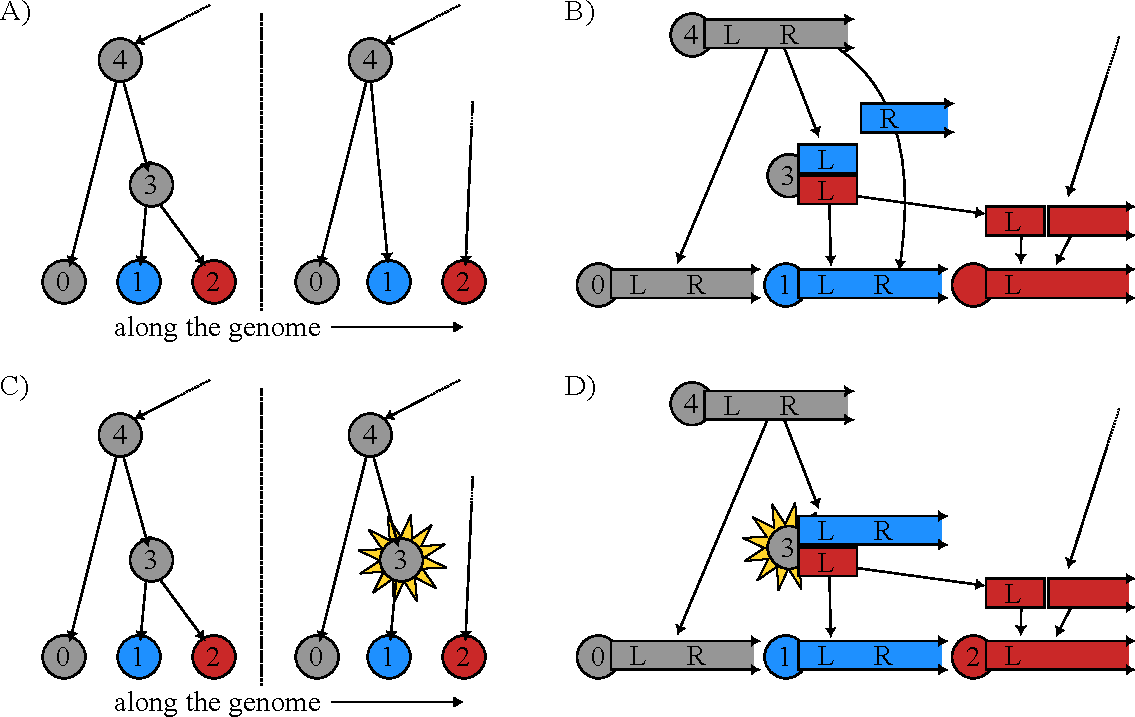
\includegraphics[width=0.9\textwidth]{conceptual_figure.pdf}
    \end{center}
    \caption{
        A simple example showing the basic idea
        (described in more detail in the text):
        \textbf{(A)} a small portion of a tree sequence without unary nodes;
        \textbf{(B)} the implied inheritance pattern of the two portions of the haplotype carried by ancestral node 4,
        labeled $L$ and $R$;
        \textbf{(C)} marginal trees with a unary node added,
        which produces \textbf{(D)} a more parsimonious haplotype inheritance pattern
        (that also includes fewer edges).
        \label{fig:conceptual}
    }
\end{figure}

%\subsection{Extend Edges}
%	\comment{Should we keep a brief section about the original extend edges? If yes, some notes are below.}
%    We do so by identifying short paths (2 edges) in a tree.
%    If neighboring trees contain edges with 
%    identical ancestor (parent) and descendant (child) nodes, 
%    we assume that there is implied coalescence of haplotypes between nodes, 
%    and we will extend the path's edges to the neighboring tree \ref{fig:extending_diagram}.
%  	In more concrete terms, for a tree $T_k$ in the tree sequence $\T$ 
%    suppose there exists a path which contains a node $3$,
%    with parent and child nodes $4$ and $0$, respectively.
%    If there is an edge between the nodes $4$ and $0$ in trees 
%    $T_{k+1}$ (or $T_{k-1}$),
%    then we wish to extend the edges $4\to 3$ and $3\to 0$ 
%    into tree $T_{k+1}$ and then remove the edge $4 \to 0$ from $T_{k+1}$. 
%    This action reduces the length of $4 \to 0$ on the genome,
%    and in some cases, completely removes the edge. 
%    We now perform this action on all such ancestral paths 
%    over the entire tree sequence.
%    With algorithm \ref{alg:edge} we only extend existing edges
%    \comment{Note possible change pending algorithm change}
%    over a larger interval on the genome,
%    and remove unnecessary edges in the process.

\section{Methods}

\subsection{Notation and terminology}

We work with the \emph{succinct tree sequence} representation of the ARG (henceforth, ``tree sequence''),
to take advantage of the extensive, stable, and well-documented set of open-source tools
available in \tskit{} \citep{tskit}, 
and our terminology and notation follows \citet{ralph2020efficiently}.
For our purposes here,
a tree sequence $\T = (N, E)$ contains a set of \emph{nodes} $N$ 
which represent ancestral segments of genome,
and \emph{edges} $E$ which represent relationships between nodes over different regions of the genome.
Each node $n \in N$ has a \emph{time} $t_n$,
which is the amount of time in the past that the individual who carried that segment of genome lived.
Some nodes are \emph{samples}, meaning that we know them from data. 
Typically, samples are exclusively leaves of $\T$, however it is not the case that all samples are leaves.
Each edge $e \in E$ describes inheritance between a parent node $p_e$ and child node $c_e$,
over a segment of genome $[\ell_e, r_e)$.
(The tree sequence includes substantially more information, including genotypes, that we will not use in this paper.)
Suppose that the unique elements of the set of left and right edge endpoints
are $0 = a_0 < a_1 < \cdots < a_{n} = L$, where $L$ is the length of the genome.
Using this information, one can construct the sequence of 
trees $\left(T_1,...,T_{n}\right)$ that describe how the nodes are related to each other along the genome:
each $T_k$ is a tree whose nodes are in $N$
and that describes relationships on the half-open interval $[a_{k-1}, a_k)$.
Not all nodes appear in each tree,
and we say $n \in T_k$ for a node $n$ if the tree $T_k$ describes at least one parent-child relationship
for node $n$.

\subsection{An algorithm to extend haplotypes}

% Description of algorithm
Given a tree sequence, our goal is to
identify areas of implied inheritance of haplotypes.
Generalizing from \figref{fig:extending_diagram},
we do this by identifying paths of inheritance that are shared across a sequence of marginal trees
but for which some of the intermediate nodes are missing.
Concretely, suppose that 
if in tree $T_k$ there is a chain of inheritance
$p \to u_1 \to \cdots \to u_m \to c$
(where $a \to b$ denotes a parent-child relationship)
and in tree $T_{k+1}$ there is a chain of inheritance
$p \to v_1 \to \cdots \to v_n \to c$,
where $\{u_i\}_{i=1}^m$ and $\{v_j\}_{j=1}^n$ are disjoint.
This situation implies that $c$ inherited from $p$ over the entire interval $[a_{k-1}, a_{k+1})$,
so it seems reasonable to assume that $c$ has inherited from $p$ \emph{along the same path} for that entire interval.
In other words, the intermediate nodes $\{u_i\}$ should also lie on the path from $c$ to $p$ in tree $T_{k+1}$,
and conversely the nodes $\{v_j\}$ should lie on that path in tree $T_k$.
Of course, this does not always make sense --
for instance, if $u_i$ is already represented somewhere else in $T_{k+1}$,
or if $t_{u_i} = t_{v_j}$, for some $i$ and $j$,
for which the intermediate nodes are not in the other tree.
So, we restrict our attention to pairs of such paths in adjacent trees
for which
$u_i \notin T_{k+1}$ for all $1 \le i \le m$,
$v_j \notin T_k$ for all $1 \le j \le n$,
and the times of the nodes $\{u_i\}$ and $\{v_j\}$ are unique.
Call a pair of such paths \emph{mergeable}.
So, the goal of our algorithm is to iterate over trees,
identify mergeable pairs of paths,
and then extend the nodes $\{u_i\}$ to $T_{k+1}$.
(We also extend $\{v_j\}$ to $T_k$, but on a backwards pass.)

\begin{figure}[!ht]
\begin{center}
	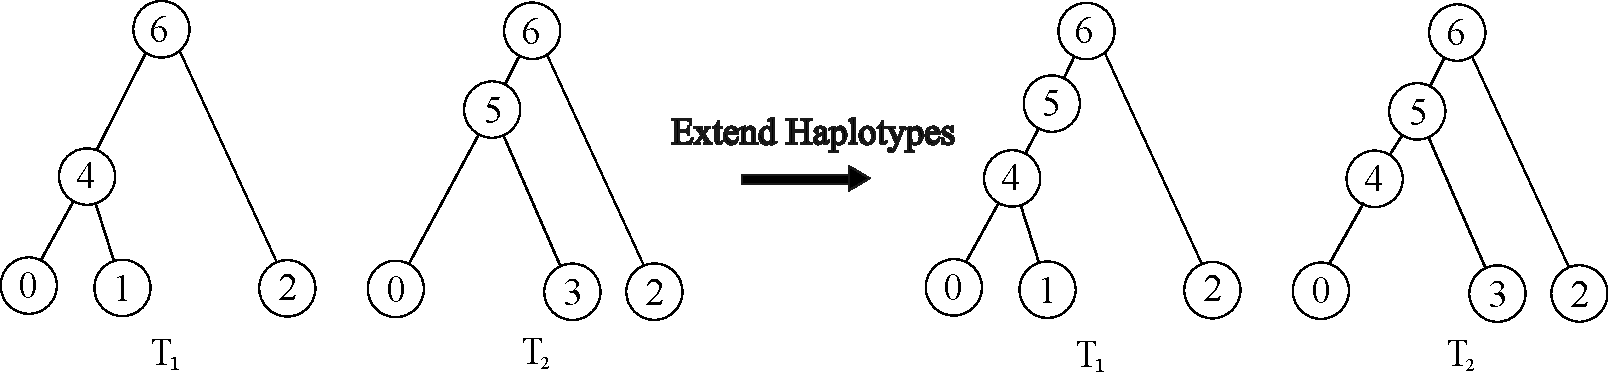
\includegraphics[width=5in]{edge_extend_method.pdf}
\end{center}
\caption{A visualization of the \textit{extend haplotypes} method. Given two neighboring trees $T_1$ and $T_2$, there exists paths from root node $6$ to sample node $0$. $T_1$ contains the path $6\to 4\to 0$ while $T_2$ has path $6\to 5\to 0$. The intermediate nodes $4$ and $5$ do not appear in $T_2$ and $T_1$ respectively, and so we consider these two paths \textit{mergeable}. The extend haplotypes method joins these two paths, constructing the merged path $6\to 5\to 4\to 0$ for both $T_1$ and $T_2$. This new path extends the edge $4\to 0$ to $T_2$ as well as constructs a new edge $5\to 4$ in the tree sequence.
    \label{fig:extending_diagram}
}
\end{figure}

A relatively efficient algorithm to do this is described in \algorithmref{alg:extend}, 
and implemented in \tskit{} as \texttt{extend\_haplotypes}.
The algorithm considers each tree transition from $T_k$ to $T_{k+1}$ in turn, updating its internal state
(which includes possibly modifying $T_k$) as it goes.
Suppose we are at the transition from tree $T_k$ to tree $T_{k+1}$,
which is done by first removing a set of edges $O$
and then adding another set of edges $I$.
$O$ defines a sub-forest $F_O$ of $T_k$,
and $I$ defines a sub-forest $F_I$ of $T_{k+1}$.
The key step in the algorithm is to determine whether the pair of paths
that terminate in a given node in two adjacent trees are mergeable,
\algorithmref{alg:mergeable}, which works as follows.
If a pair of paths is mergeable,
then the edges of the two paths must lie in $O$ and $I$, respectively.
Suppose an edge in $O$ has child $c$.
To see if $c$ is the base of a pair of mergeable paths,
the algorithm traverses up from $c$ in both $F_O$ and $F_I$;
terminating if a node in the other tree is found
(i.e., if the node traversed in $F_O$ is in $T_{k+1}$ or if the node traversed in $F_I$ is in $T_k$)
or if a pair of traversed nodes have the same time.
If these two traversals end in the same node $p$, the paths are mergeable.
Iterating over all edges in $O$ will thus find all mergeable pairs of paths.
There is often more than one pair of mergeable paths in a tree transition;
so, the algorithm merges pairs of mergeable paths,
starting with pairs that add the smallest number of new edges,
until no more are found.


\algorithmref{alg:extend} simplifies the algorithm in several ways for the sake of clarity --
for instance, the bookeeping required to keep track of $T_k$ and $T_{k+1}$ is omitted.
Furthermore, as described the algorithm does one left-to-right pass over the tree sequence;
in practice we do repeated passes in both directions until no changes can be made.
The main step that is omitted is a description of the \texttt{merge} operation,
which performs the actual extending of haplotypes.
This algorithm is essentially the same as \texttt{mergeable} in \algorithmref{alg:mergeable},
except with additional bookkeeping.
Roughly speaking, the algorithm
traverses up from the shared base node $c$,
doing the appropriate operations to insert the nodes along the path found in $T_k$
into the path in $T_{k+1}$.
To do this, some edges that end at $a_k$ will be extended to end at $a_{k+1}$;
some edges that begin at $a_k$ will be postponed to begin at $a_{k+1}$,
and some entirely new edges may be added, see \figref{fig:extending_diagram}.
Furthermore, the trees $T_k$ and $T_{k+1}$ (and corresponding forests $F_O$ and $F_I$)
need to be updated.


\begin{algorithm2e}[!ht]
	\SetStartEndCondition{ }{}{}%
	\SetKwProg{Fn}{def}{\string:}{}
	\SetKwFunction{Range}{range}%%
	\SetKw{KwTo}{in}
	\SetKwFor{For}{for}{\string:}{}%
	\SetKwIF{If}{ElseIf}{Else}{if}{:}{elif}{else:}{}%
	\SetKwFor{While}{while}{:}{fintq}%
	\SetKw{Break}{break}
	\newcommand\forcond{$i$ \KwTo\Range{$n$}}
	\AlgoDontDisplayBlockMarkers\SetAlgoNoEnd\SetAlgoNoLine%
    \caption{
        Given a node $c$, trees $T_O$ and $T_I$,
        and sub-forests $F_O$ and $F_I$
        such that removing $F_O$ and adding $F_I$ turns $T_O$ into $T_I$,
        check to see if the paths upwards from $c$ in $T_O$ and $T_I$ are mergeable.
        If the paths are mergeable then this returns the number of new edges
        that would be added by extending the path from $T_O$ to $T_I$;
        otherwise, returns $\infty$.
        Let $P_O[n]$ and $P_I[n]$ be the parents of node $n$
        in the set of edges to be removed and added, respectively
        (i.e., in $F_O$ and $F_I$).
    }
	\label{alg:mergeable}
	\SetKwFunction{mergeable}{Mergeable}
	\DontPrintSemicolon
    \Fn{\mergeable($c$, $T_O$, $T_I$)}{
        $p_i = P_I[c]$\;
        $t_i = t[p_i]$\;
        $p_o = P_O[c]$\;
        $t_o = t[p_o]$\;
        $n_e = n = 0$\;
        \While{\tn{True}}{
            $y_i = (p_i \neq NULL)
                \text{ and } (p_i \notin T_O)
                \text{ and } (t_i < t_o)$ \;
            $y_o = (p_o \neq NULL)
                \text{ and } (p_o \notin T_I)
                \text{ and } (t_o < t_i)$ \;
            \If{not ($y_i$ or $y_o$)}{ \Break\; }
            \eIf{$y_i$}{
                \If{$P_I[c] \neq p_i$ and $P_O[c] \neq p_i$}{
                    $n_e += 1$\;
                }
                $c = p_i$\;
                $p_i = P_I[p_i]$\;
                $t_i = \text{ if }(p_i = NULL)\text{ then }\infty\text{ else }t[p_i]$\;
            }{
                \If{$P_I[c] \neq p_o$ and $P_O[c] \neq p_o$}{
                    $n_e += 1$\;
                }
                $c = p_o$\;
                $p_o = P_O[p_o]$\;
                $t_o = \text{ if }(p_o = NULL)\text{ then }\infty\text{ else }t[p_o]$\;
                $n += 1$\;
            }
        }
        \If{$n = 0$ or $p_i \neq p_o$ or $p_i = NULL$}{
            $n_e = \infty$\;
        }
        \KwRet{$n_e$}\;
    }
\end{algorithm2e}

\begin{algorithm2e}[!ht]
	\SetStartEndCondition{ }{}{}%
	\SetKwProg{Fn}{def}{\string:}{}
	\SetKwFunction{Range}{range}%%
	\SetKw{KwTo}{in}
	\SetKwFor{For}{for}{\string:}{}%
	\SetKwIF{If}{ElseIf}{Else}{if}{:}{elif}{else:}{}%
	\SetKwFor{While}{while}{:}{fintq}%
	\SetKw{Break}{break}
	\newcommand\forcond{$i$ \KwTo\Range{$n$}}
	\AlgoDontDisplayBlockMarkers\SetAlgoNoEnd\SetAlgoNoLine%
    \caption{Extend haplotypes.}
	\label{alg:extend}
	\SetKwFunction{mergeable}{Mergeable}
	\SetKwFunction{merge}{Merge}
	\SetKwFunction{extend}{ExtendHaplotypes}
	\DontPrintSemicolon
    \Fn{\extend($\T$)}{
        \For{$k$ in $1 \ldots N$}{
            $M = 0$\;
            $M' = \infty$\;
            \While{$M < \infty$}{
                \For{$e \in O_k$}{
                    $m$ = \mergeable($c_e$, $T_k$, $T_{k+1}$)\;
                    \eIf{$m < M$}{
                        \merge($c_e$, $T_k$, $T_{k+1}$)\;
                    }{
                        $M' = \min(m, M)$\;
                    }
                }
                $M = M'$\;
                $M' = \infty$\;
            }
        }
    }
\end{algorithm2e}

Since the algorithm needs to take multiple passes over the tree sequence
in each direction,
an important practical question for this algorithm is:
how passes do we need to do?
The algorithm is monotone (spans of ancestral nodes only increase),
so it is guaranteed to require only a finite number of passes,
but it is also not hard to construct pathological cases that require an arbitrary number of passes.
Counting edges for every iteration suggest that only at most five iterations are needed before the algorithm terminates.
Indeed, for even larger sequences \tabref{tab:edge-counts}
shows that 99\% of all changes to an ARG occur after the first iteration,
with the algorithm completing after four iterations. 


\subsection{Dissimilarity between ARGs}
% * How to measure agreement that includes haplotypes
% * Definition and Algorithm
% * Supp fig: runtime ~ # trees, samples
% * fig: how add edges reduces discrepancy (RESULTS)
%       - compare to tsinfer
% * Show: how add edges reduces discrepancy (RESULTS)

If we begin with a tree sequence containing unary nodes,
it is straightforward to remove the portions of each node's span on which it is unary,
apply \algorithmref{alg:extend},
and quantify how much node span was correctly or incorrectly added.
However, we are also interested in whether \algorithmref{alg:extend}
improves \emph{inferred} tree sequences.
Since we are not aware of any current methods for measuring (dis)agreement between tree sequences
that take into account haplotype identity,
we define a measure of \emph{dissimilarity} to quantify this.
The method is implemented in the \texttt{tscompare} package.

It is helpful to first describe what we compute in the simple case.
\figref[C\&D]{fig:node-spans} shows the spans for each node in three tree sequences:
for each node the total span in a ``true'' tree sequence, 
given by the line,
that was simulated with \msprime \citep{kelleher2016efficient,baumdicker2021efficient}
in a way that included spans over which nodes are unary in the output
(by setting \texttt{coalescing\_segments\_only} to False).
\figref[C]{fig:node-spans} shows the span of each node after \emph{simplifying} the tree sequence 
\citep{kelleher2018efficient},
which removes all unary nodes from all trees
thus reducing the node spans for some nodes in the sequence.
In \figref[D]{fig:node-spans}
is the span of the node after applying \algorithmref{alg:extend}
to the simplified tree sequence.
\algorithmref{alg:extend} cannot reduce node span, resulting in node spans 
from the extended tree sequence that are closer in value to the ``true'' tree sequence. 
\figref[B]{fig:node-spans} shows how much of this span is incorrect:
for each node, it gives the amount of span
that is incorrect (i.e., not present in the original tree sequence) % NSP-22NOV: it seems a bit odd that this panel (B) is not on a log scale while all the others are
over the total amount of span added after running \algorithmref{alg:extend}.
The values in these plots
therefore quantify how much the ancestral haplotypes represented by each node
were correctly, and incorrectly, extended.
They also tell us how much of the relationships in the original tree sequence
are represented in the result. % NSP-22NOV: "relationships" of what exactly?

Now suppose that instead of comparing two tree sequences with the same set of nodes,
we wish to compare two tree sequences for which we know the sample nodes are the same
but are otherwise unclear as to the equivalency of nodes across sequences
(as for instance with a true, simulated tree sequence and one inferred from its genotypes;
in the former nodes represent actual ancestral haplotypes, and in the latter
represent hypothetical ancestors which may or may not resemble the truth).
Call the two tree sequences $T_1$ and $T_2$, which should have the same genome length
and the same set of sample nodes.
We would like to measure (a) how much of $T_1$ is found in $T_2$;
(b) how much of $T_1$ is \emph{not} found in $T_2$; and
(c) how much of $T_2$ is not found in $T_1$.
(Think of these three quantities as the size of the intersection
and two differences between the tree sequences,
thought of vaguely as sets.)
Roughly speaking, we first identify matching nodes
as those whose sets of descendant samples agree for the largest span along the genome,
and then compute for how much of their spans do their descendant samples agree (or not).

Concretely, our method can be applied to any two tree sequences,
 as in the case of \figref{fig:conceptual_discrepancy},
 where we consider the pair of trees which exist at that break point.
However, to simplify notation suppose that the two tree sequences have the same set of breakpoints
between trees,
so that $T_1^{(1)}, \ldots, T_N^{(1)}$ are the trees in $\T_1$
and $T_1^{(2)}, \ldots, T_N^{(2)}$ are the trees in $\T_2$.
For a node $n$ and tree $T$
let $S(T, n)$ denote the set of samples that inherit from $n$ in $T$,
and for a pair of nodes $n_1$ and $n_2$ with $n_1$ in $\T_1$ and $n_2$ in $\T_2$,
define
% NSP-22NOV: The notation here is hard to read when subscripted. IMO it'd be better to use bracket notation here for the indicator function,
% \mathbb{I}[ S(T_k^{(1)}, n_1) = S(T_k^{(2)}, n_2) ]
% and also in next equation for consistency.
\begin{align*}
    m(n_1, n_2)
    =
    \sum_{k=1}^N (a_k - a_{k-1}) \ind_{S(T^{(1)}_k, n_1) = S(T^{(2)}_k, n_2)}  
    % NSP-22NOV: Added a missing comma. Also the comma at the very end looks like a prime, which is confusing, so I'm removing grammatical punctuation from these non-inline equations.
\end{align*}
which is the total span over which the samples below $n_1$ in $\T_1$
matches the samples below $n_2$ in $\T_2$.
Also let
\begin{align*}
    s(\T, n) = \sum_{k=1}^N (a_k - a_{k-1}) \ind_{n \in T_k} 
\end{align*}
the total span that node $n$ is present in the marginal trees.
The \emph{similarity} between $\T_1$ and $\T_2$ is then defined to be
\begin{align*}
    \similarity(\T_1, \T_2)
    =
    \max_{\beta:N_1 \to N_2} \sum_{n \in N_1} m(n, \beta(n)) 
\end{align*}
where the maximum is over all mappings $\beta$ of nodes in $\T_1$ to nodes in $\T_2$.
(Note that multiple nodes in $\T_1$ may be mapped to the same node in $\T_2$,
and that there may be no nodes in $\T_1$ that are mapped to some nodes in $\T_2$.)
Since the maximum is independent over nodes, we may define for each node $n_1 \in \T_1$
it's \emph{best matching node} in $\T_2$ as
\begin{align*}
    \alpha(n_1) = \argmax_{n_2 \in N_2} m(n_1, n_2) 
\end{align*}
so that
\begin{align*}
    \similarity(\T_1, \T_2)
    =
    \sum_{n \in N_1} m(n, \alpha(n)) 
\end{align*}
If the best-matching node is unique, we define $\alpha(n_1)$ to be the node in $T_2$
out of those maximizing $m(n_1, n_2)$ that minimizes $|t^{(1)}_{n_1} - t^{(2)}_{n_2}|$
(and if \emph{this} is not unique, we pick an arbitrary one) --
however, this potential ambiguity does not affect the definition of $\similarity(\T_1, \T_2)$.
Let $\|\T_1\|=\sum_{n\in N_1}s(\T_1,n)$ be the total sum of nodes spans for nodes in $\T_1$.
We then define the \emph{dissimilarity} of $\T_1$ from $\T_2$ by
\begin{align*}
    \dis(\T_1, \T_2)
    =
    \sum_{n \in N_1} (s(\T_1, n) - m(n, \alpha(n))) 
    = 
    \Vert \T_1\Vert -\similarity(\T_1,\T_2),
\end{align*}
which is the proportion of total span of all nodes in $\T_1$
for which their descendant samples do \emph{not} match those of their best match in $\T_2$.

Other authors \citep[e.g.,]{kelleher2019inferring} have used
an average Robinson-Foulds distance \citep{robinson1981comparison}
as a measure of disagreement between tree sequences.
This could be computed in a very similar way:
instead of $m(n, \alpha(n))$ define
% NSP-22NOV: as before I'd suggest using \mathbb{I}[...] for the indicator function
\begin{align*}
    m'(n, \T_2) = \sum_{k=1}^N (a_k - a_{k-1}) \ind_{\exists n_2: s(T^{(2)}_k, n_2) = s(T^{(1)}_k, n)} ,
\end{align*}
the total span over which there is \emph{some} node in $\T_2$ whose set of descendant samples
matches $s(T_1,n)$.
Then the average Robinson-Foulds distance (averaged over locations in the genome)
is
\begin{align*}
    \frac{1}{L} \left( \sum_{n_1 \in N_1} m'(n_1, \T_2)  + \sum_{n_2 \in N_2} m'(n_2, \T_1) \right).
\end{align*}
In other words, we require a node in $\T_1$ to match the \emph{same} node in $\T_2$
across all trees, but average Robinson-Foulds distance allows a different node to match
on each tree.
The other differences are that \emph{average} Robinson-Foulds distance
normalizes by sequence length, and is symmetrized.
Robinson-Foulds distance between two trees
was defined by \citet{robinson1981comparison}
to the minimum number of edge contraction/expansion operations needed to move
from one tree to the other
(which they then show is equal to the number of edges that induce different splits on the labels).
A similar metric on tree sequences could possibly be defined
using subgraph-prune-and-regraft moves \citet{deng2024robust}.

The dissimilarity $\dis(\T_1, \T_2)$ measures disagreement between \emph{topologies},
but not times.
If the tree sequence is dated, we can naturally use the ``best match'' $\alpha$
to also compare times,
for instance by returning the weighted root-mean-squared error on inferred times as
\begin{align}\label{eqn:wrmse}
    \text{wRMSE}_t(\T_1, \T_2)
    = \sqrt{\frac{
        \sum_{n \in N_1} s(\T_1,n) \left(\log\left(1+ t^{(1)}_n\right) - \log\left(1+ t^{(2)}_{\alpha(n)}\right) \right)^2 
    }{
        \Vert{\T_1}\Vert
    } } .
\end{align}
The mean is computed weighting by node span, so that a dating error
is more impactful for a node with a longer span. 

The implementation of this method in \texttt{tscompare}
additionally produces relative values:
the ancestral recombination graph Robinson-Foulds value (relative dissimilarity) and true proportion represented. 
The \emph{ARG Robinson-Foulds} (ARF) is defined to be the dissimilarity proportional
 to the total span of nodes in $\T_1$,
 \begin{align}\label{eqn:dissimilarity}
 	\operatorname{ARF}(\T_1,\T_2)=\frac{\dis(\T_1,\T_2)}{\Vert \T_1 \Vert}
 	=1-\frac{\similarity(\T_1,\T_2)}{\Vert \T_1\Vert}.
\end{align}
The \emph{true proportion represented} (TPR) is similarity between two trees relative 
to the total span of nodes in $\T_2$,
\begin{align}\label{eqn:true-proportion}
	\operatorname{TPR}(\T_1,\T_2) = \frac{\similarity(\T_1,\T_2)}
	{\Vert \T_2\Vert}.
\end{align}
The outputs framed as proportions relative to one of the given tree sequences is more easily understood
for comparing pairs of tree sequences than the original dissimilarity and similarity, whose units are length of spans.
We compute dissimilarity and ARF of two tree sequences in \figref{fig:conceptual_discrepancy}.

\begin{figure}[!ht]
	\begin{center}
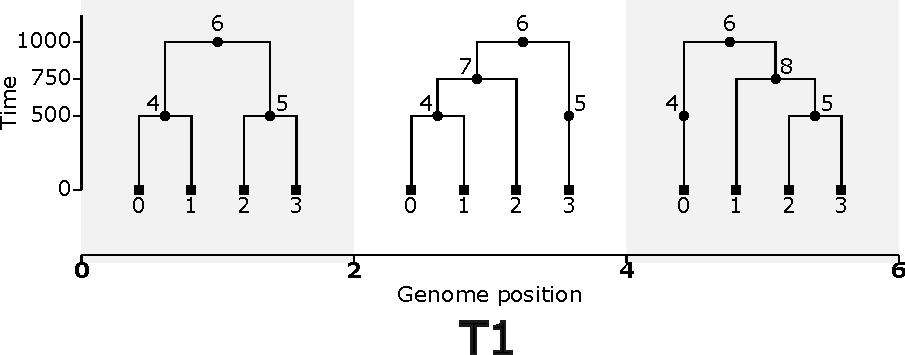
\includegraphics[height=1.5in, width=3in]{discrepancy_func_method_t1.pdf}
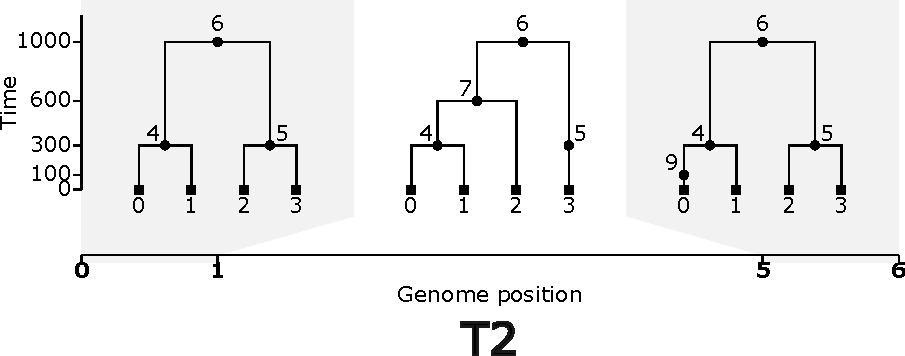
\includegraphics[height=1.5in, width=3in]{discrepancy_function_method_t2.pdf}
    \caption{
        For two tree sequences $T1$ and $T2$ the \emph{dissimilarity}, $\dis(T1,T2)$, matches nodes in $T1$ to nodes in $T2$
        based on identical sample sets.
        In this example, node $8$ has no match in $T2$ as there are no nodes in $T2$ with sample set $\left\{1,2,3\right\}$.
        Node $4$ has no match on $[4,5)$ and matches with node $9$ on $[5,6)$. Thus the maximal mapping for 4 should be to itself. On the rest of the genome, all of nodes match with their identical counterpart.
        This makes the dissimilarity $\dis(T1,T2)=3$ and $\operatorname{ARF}(T1,T2)=\frac{3}{46}$.
        \label{fig:conceptual_discrepancy}
    }
	\end{center}
\end{figure}

%%%%%%%%%%%%%%%%%%%%%%%%%%%%%%
\subsection{Simulations}

To do this, we simulate ARGs containing full haplotypes using \msprime's 
option \texttt{coalescing\_segments\_only} set to False.
Although \msprime\ simulates many events that do not create a coalescence in some marginal tree,
it only outputs information for nodes which contain a coalescence
(i.e., are the MRCA of some pair of samples at some point on the genome).
Furthermore, by default it only outputs those segments of the genome
on which there is a coalescence.
Said another way, by default all ancestral nodes in the ARG
output by \msprime\ are the MRCA of some pair of samples at every point in the genome
on which they are represented.
However, here we are interested in those segments of genome
on which the nodes are \emph{not} coalescent;
i.e., where they are unary in the marginal trees.
More concretely, we hope to recover those portions of ancestral haplotypes
on which the nodes are unary, but adjacent to a region of the genome where the node is not unary.
For instance, if a lineage carrying an ancestral segment of genome that spans $[a, c)$
coalesces with another spanning $[b, d)$, with $a < b < c < d$,
then the resulting node is only coalescent on $[b, c)$ but we hope using this algorithm
to extend the node's span to $[a, b)$ and $[c, d)$
(on which the node is unary).
However, following this example, the first lineage might carry a segment $[x, y)$
that is disjoint from the coalescent segment $[a, d)$.
We call these segments ``isolated non-coalescent segments'';
they have also been called ``trapped unary spans'' \citep[by][]{XXX}.
Such isolated segments will not be recovered by our algorithm,
and would likely be unrecoverable by any other method.
So, when evaluating what proportion of the true ARG is represented in an inferred ARG
we omit these isolated non-coalescent segments.
To give an idea of what proportion of the full spans of ancestral nodes
these isolated non-coalescent segments represent,
a simulation of 1000 samples
with genome length $5\times 10^7$, recombination rate $10^{-8}$, and population size $10^4$
has about half the total span of all nodes in isolated, non-coalescent segments.
For more discussion of these segments, see \citet{baumdicker2021efficient}.

We used simulations of several scenarios.
To include the effects of heterogeneous recombination rate,
in some we used stdpopsim \citep{stdpopsim} 
to simulate chromosome 1 of \textit{Canis familiaris}
using the CanFam3 genetic map from \citet{campell2016}.
\emph{``Constant dog''} simulations simulated this chromosome in a 
population of (constant) size $10^4$.
\emph{``Expanding dog''} simulations were similar, but
used a discrete-time Wright--Fisher model to simulate
a small population of 100 that expanded to 1,000 individuals ten generations ago,
which then doubled every generation to reach 512,000 individuals.
All jobs for which runtime was recorded were executed on an Intel Xeon Gold 6148 processor.
 Additionally, we compare accuracy between sequences modified from a ``true'' tree sequence
 using our dissimilarity methods. 
 These tree sequences have a population of 1,000 and recombination rate of $10^{-8}$ with samples ranging from 10 to 1,000 and genome length ranging from $10^6$ to $5\times 10^7$.


\section{Results}

% Outline:
% 1. benchmarking: edge reduction and runtime
% 2. correctness:

%% TO DO:
%% 1. Discuss trapped unary spans more
%% 2. Discuss the comparison between tsinfer and extend haplotypes
%% 3. Add more figures 
%%	- (Edge counts between tsinfer and extend haplotypes)
%%	- Average Edge counts per iterations
%% 4. Discuss figures about total edge span added in both recombination and gene conversion events
%% 5. Discuss the figures on edge reduction (include #3 part 1.)

%%%%%%%%%%%%%%%%%%%%%%%
\subsection{Tree sequence compression and computation}


In the simple example in \figref{fig:conceptual},
extending haplotypes replaces three edges
($0 \to 3$ and $3 \to 4$ on the left tree, and $0 \to 4$ on the right tree)
by two edges ($0 \to 3$ and $3 \to 4$ on both trees).
If all edge endpoints were unique, then we'd expect \emph{every} edge to be extendable
on one of its ends
(except those pendant to the root and some of those adjacent to chromosome ends),
leading to a reduction in number of edges by a third.
Experiments with an earlier version of the algorithm showed that
if we only extend haplotypes on ``paths of length 1'', 
then the hypothesized reduction of 1/3 is achieved for long sequences. % NSP-22NOV: is this sentence mentioning the earlier algorithm necessary?
It is possible for \algorithmref{alg:extend} to add edges, as in \figref{fig:extending_diagram},
but we still expect the number of edges to decrease by more than 1/3.
Indeed,
\figref{fig:speed_and_edges} shows that \algorithmref{alg:extend} nearly cuts the number of edges
in half, as long as the sequence is long enough.

\begin{figure}
    \centering
    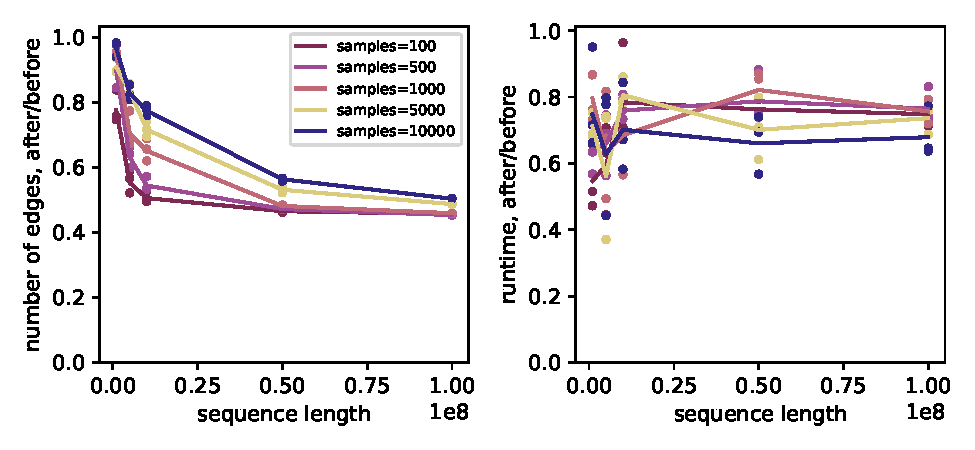
\includegraphics{benchmarks/one_pop_results_ratios}
    \caption{
        Ratio of
        \textbf{(A)} number of edges, and
        \textbf{(B)} runtime for computing Tajima's $D$;
        before and after extending haplotypes.
        For instance, extending haplotypes reduces number of edges by about 50\%
        and statistic computation runtime by about 20\%
        for long sequences.
        Horizontal axis shows sequence length;
        colors show numbers of samples;
        with lines showing averages across replicates.
        The original tree sequence was simulated with the ``expanding dog'' expanding population
        and subset to various sizes;
        see Methods for details. 
        Absolute values are shown in Supplementary \figref{fig:speed_and_edges_other}.
        \label{fig:speed_and_edges}
    }
\end{figure}

This reduction in edges can also lead to a reduction in computation time for
algorithms using the succinct tree sequence data structure.
Indeed, \figref{fig:speed_and_edges} shows that computation time is reduced by 10--20\%
for a typical statistic (here, Tajima's $D$),
computed in an efficient incremental manner along the genome as implemented in \tskit.
As described in \citet{ralph2020efficiently}, for these incremental algorithms
the addition or removal of an edge requires updates
to the state of the parent node and all nodes above it.
Extending haplotypes yields a tree sequence with fewer edge removals and insertions, 
and thus requires fewer traversals to the roots.

Supplementary \figref{fig:speed_and_edges_constant} shows these results are not specific
to the demographic scenario.
Supplementary Figures~\ref{fig:speed_and_edges_other}
and~\ref{fig:speed_and_edges_other_constant}
also show that our implementation of \algorithmref{alg:extend} is quite efficient,
running at chromosome scale in seconds to minutes for hundreds or thousands of samples,
or minutes to hours for tens of thousands of samples


%%%%%%%%%%%%%%%%%%%%%%%
\subsection{Accuracy with true trees}

Our next task is to confirm that the haplotypes extended by \algorithmref{alg:extend}
are indeed correct -- i.e., that in addition to compression, we are also gaining information.
To do this, 
we simulate ARGs containing full haplotypes using \msprime{},
apply the simplification algorithm to reduce these so that there are no unary nodes
(i.e., any node present in a marginal tree is a coalescent node or a sample),
and then apply \algorithmref{alg:extend} to the result
(see Methods for more detail).
The method can potentially extend the spans of each node
(additional span over which the node will be unary);
and we can quantify how much of these extended spans were in the original ARG
(and thus correctly extended).

%$msprime.sim_ancestry(1000, sequence_length=5e7, recombination_rate=1e-8, population_size=1e4, coalescing_segments_only=False, random_seed=1)$
%From the above output we see that ratio of unary span bordering coalescing between 
%- ExtendPaths/Truth = 0.4917
%- ExtendEdges/Truth = 0.27828
%
%The trapped unary span of our ground truth is 49\% of the TS.
%
%Total unary span bordering coalescing: 255151996720.0 (51.0\%)
%Total trapped unary span: 245038231157.0 (49.0\%)
%Total coalescing span: 99950000000.0
%Total unary span bordering coalescing: 125466159245.0 (100.0\%)
%Total trapped unary span: 0.0 (0.0\%)
%Total coalescing span: 99950000000.0

As seen in \figref{fig:node-spans},
the vast majority of span added by extending haplotypes is correct.
In this example (which is typical),
99\% of all added span is correct;
95\% of nodes have no incorrectly added span;
and those incorrectly added spans are nearly always a small fraction of the original span.
The added information is significant:
the algorithm typically increases spans (i.e., lengths of ancestral haplotypes)
by around 50\%.

\begin{figure}[!bht]
	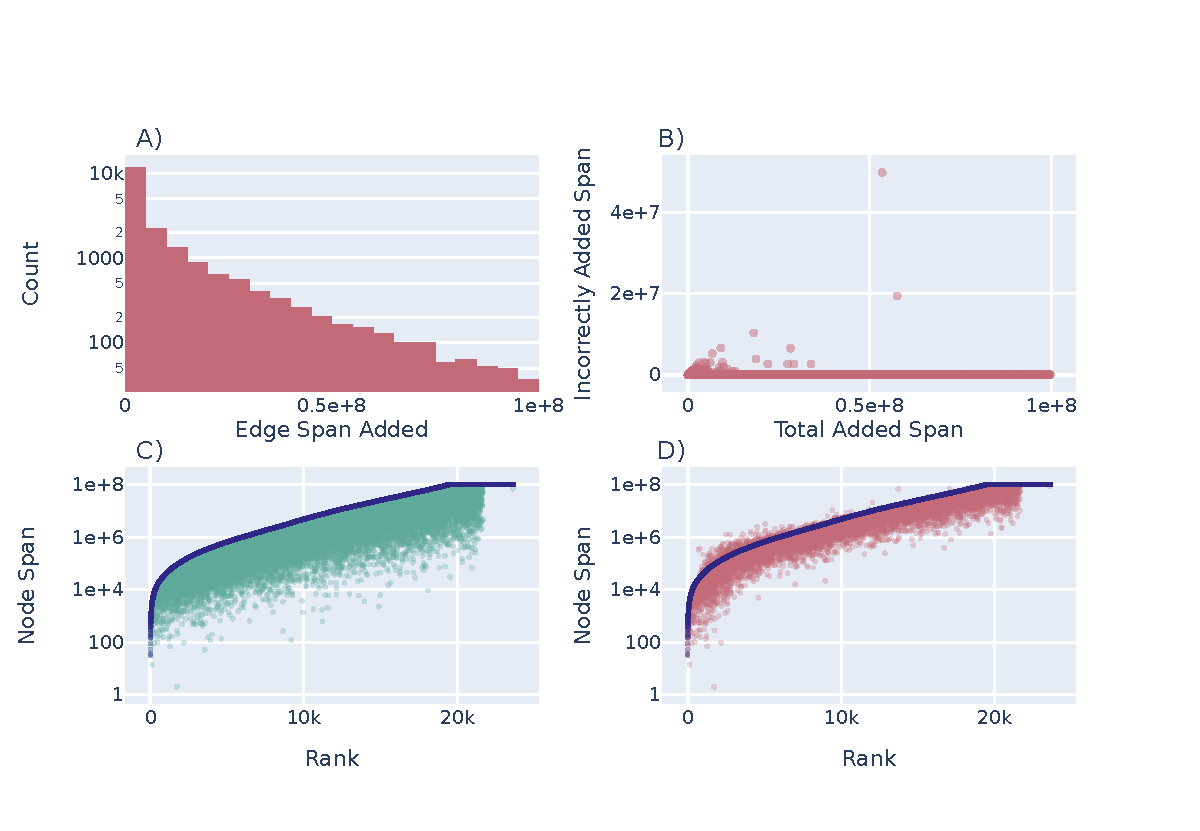
\includegraphics{newplots_wo_ee/figure-4.pdf}
	\caption{
        The effect of extending haplotypes on per-node spans
        in an ARG simulated with $10^4$ diploid samples, $10^4$ population, and 
        recombination rate of $10^{-8}$ on a sequence of length $10^8$.
        \textbf{(A)}
        Distribution of total amount of span added across nodes by \algorithmref{alg:extend};
        note the log scale on the $y$ axis.
        \textbf{(B)}
        Amount of incorrectly added span, plotted against total span, by node.
        95\% of nodes have no incorrect span; of the remainder,
        nearly all have less than 5\% incorrectly added;
        see Supplementary \figref{fig:incorrect_ratio}.
        Plots \textbf{(C)} and \textbf{(D)} show total spans per node,
        ordered by total span in the original ARG (which includes unary nodes).
        Dark blue dots in both show the spans in this original ARG.
        In \textbf{(C)}, lighter green dots show
        span after removing unary spans using \textit{simplify},
        while in \textbf{(D)},
        lighter red dots show span after extending haplotypes,
        i.e., applying \algorithmref{alg:extend} to the simplified ARG.
    }
	\label{fig:node-spans}
\end{figure}

These statistics are also reflected at the genomic scale, using measures of dissimilarity.
Line ``SE'' in \figref{fig:dissimilarity} shows total amounts of span removed by simplification
and re-inferred by \algorithmref{alg:extend} (correctly and incorrectly).
(Lines labeled with ``I'' involve re-inference of the ARG; discussed next.)
The top row shows the proportion of the given ARG that does not match the original (ARF),
showing that the total amount of mis-matching span
produced by extending haplotypes is very small ($\approx 1\%$).
(Simplification does not produce dissimilarity.)
The bottom row shows the proportion of the original ARG that is represented in the given ARG (TRP).
This shows that a large proportion of the ARG can be removed by simplification,
indicating that coalescent nodes are unary
over a substantial portion of their spans.
(Since the \texttt{simplify} operations removes these unary portions of haplotypes,
the ``simplified'' line (``S'') on the right of Figure~\ref{fig:dissimilarity} shows
the proportion of nodes' spans on which they are not unary.)
However, \algorithmref{alg:extend} can correctly replace most of these portions of haplotypes,
especially with larger sample sizes and sequence lengths
(the ``simplified--extended'' line; ``SE'').
For instance, with 1,000 samples and a $5 \times 10^7$bp genome,
haplotypes are unary on about half their spans (on average),
and extending haplotypes can infer more than half of this span from coalescent information only.



\begin{figure}[!hbt]
	\begin{center}
        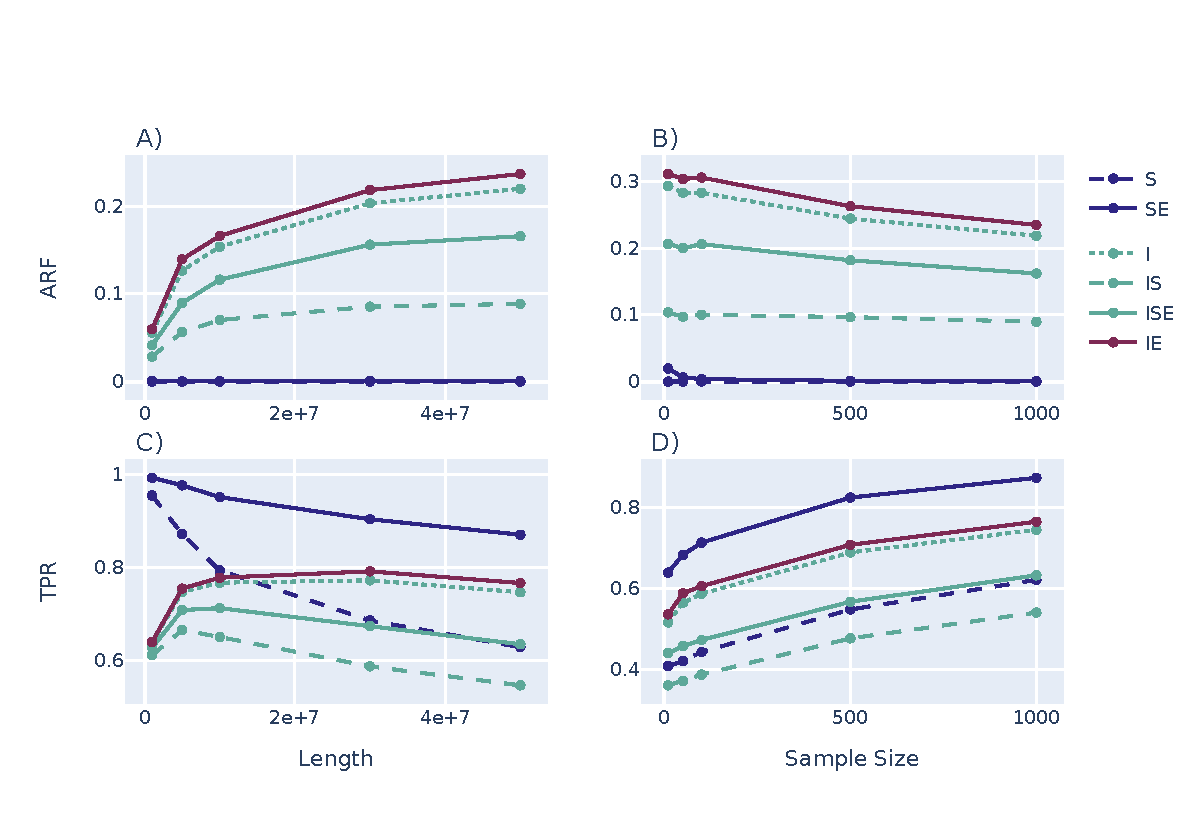
\includegraphics[width=\textwidth]{figure5.pdf}
	\end{center}
    \caption{
        Accuracy and sensitivity of extended haplotypes
        across a range of sample sizes, on a sequence of length $5\times10^7$ (top)
        and sequence lengths, with 1,000 diploid samples (bottom).
        For each, a simulated ARG containing unary haplotype spans
        was (i) \emph{simplified}, removing the unary spans,
        and (ii) \emph{inferred}, using \tsinfer{} on genotypes;
        then each of these had its haplotypes \emph{extended}.
        The inferred, then simplified, ARG is also shown.
        \textbf{Top row:} ARF, the dissimilarity to the true ARG,
        as proportion of haplotypes that are not represented in the true ARG
        (\eqnref{eqn:dissimilarity}).
        \textbf{Bottom row:} TPR, agreement to the true ARG
        as proportion of the true ARG that is represented.
        }     
    \label{fig:dissimilarity}
\end{figure}


%%%%%%%%%%%%%%%%%%
\subsection{Inferred ARGs}

So far, we have demonstrated that there is potentially ample information
in the coalescent-only trees to extend haplotypes.
Does this work with \emph{inferred} ARGs?
Indeed, most ARG inference methods provide inferred ARGS already containing unary nodes; % NSP-22NOV: this isn't true I don't think-- isn't it just tsinfer?
to what degree are they taking advantage of this information already?
Here, we study the behavior of \tsinfer{}, which produces unary nodes as a
byproduct of its inference algorithm,
and leave a comparison across other ARG inference methods for future work.
We simulated ARGs containing unary-spanning haplotypes (as above), then
re-inferred ARGs from the associated genotypes and performed various operations
on the results.
% NSP-22NOV: do we need to define TS simplification here (or earlier?)

First, \figref{fig:dissimilarity} shows that \tsinfer{}
has a substantial portion of already--extended haplotypes:
comparing the ``inferred'' (``I''; dotted green) line to the ``inferred-simplified'' (``IS''; dashed green) line
we see that inclusion of these unary spans increases the amount of correctly inferred material
by around 20\% (bottom panels),
but that roughly 10\% of the unary spans in the inferred ARG are incorrect (top panels).
Furthermore, comparing to the inferred-extend(``IE''; red) line, we see that extending the tree sequence output with tsinfer adds relatively little span.
Applying \algorithmref{alg:extend} to the inferred-and-then-simplified ARG
(``ISE''; solid green line)
produces an ARG with both less correct and incorrect span.
Additionally, the ``IE'' and ``ISE'' ARGs 
contain approximately the same number of edges (difference of $\approx 1\%$).
It is also helpful to note that accuracy
(i.e., proportion of the true ARG that is inferred; bottom panels)
greatly increases with larger sample sizes,
possibly due to resolution of polytomies.
(Recall that due to computational constraints,
``correct'' and ``incorrect'' spans are determined here by \emph{exact} match
of subtending samples.)

%reporting proportions of correct and incorrect haplotype spans in Figure~\ref{fig:dissimilarity}.
%Main points: in \figref{fig:dissimilarity}
%(green line) tsinfer gets a lot right (above 60\% with 1000 samples; bottom-right plot)
%    and does a lot better with more samples;
%    also, gets 10\%--25\% wrong (left panels)
%    with longer sequence, larger proportion is wrong (bottom-left panel)
%(red dotted)
%    simplifying removes a lot of the wrong stuff
%    but also a lot of the right stuff
%(red solid)
%    similarly extending the simplified one adds a bunch of right and also wrong stuff
%    
%
%It's also interesting to  note that inference
%(see \figref{fig:inferred_edge_counts})
%(a) increases number of edges;
%(b) but inferred-simplifies have even more suggesting unary stuff is parsimonious;
%(c) but then extending reduces to below the original.


\section{Discussion}

We began this study with the observation that the simple transformation
of \figref{fig:extending_diagram} would reduce the number of edges
in the succinct tree sequence representation of the ARG.
This is essentially a recombination-based parsimony argument,
and we have shown that this line of reasoning
leads to ARGs that are substantially more compact and faster to operate on,
and that contain more complete information about true ancestral relationships. % NSP-22NOV: 'accurate' ==> 'complete' as otherwise it sounds like we're changing the topologies
These extended ancestral haplotypes manifest as unary nodes in the marginal trees.
Although a number of ARG inference methods may be taking advantage of this information,
it is our impression that this source of information is not widely appreciated.
In fact, due to the field's focus on marginal trees rather than haplotypes,
we had to develop a haplotype-aware measure of (dis)agreement between ARGs in order to study the accuracy of the proposed algorithm.

There are good reasons to think that lengthening the spans of ancestral haplotypes
could lead to substantial gains in accuracy of ARG inference.
For instance, information about inferring the age of a particular mutation
derives almost entirely from constraints at nearby, linked sites.
Extending ancestral haplotypes from one site into neighboring regions
conceptually allows information from those marginal trees
to inform age inference at that site as well.

We have also explored the degree to which \tsinfer{} already makes use of this information,
and whether this algorithm can be used to improve inference.
The results do not provide a clear ordering:
for instance, although \tsinfer-produced ARGs
have a substantial portion of correctly inferred unary haplotypes,
removing these with simplification decreases both ARF
(i.e., proportion of ``wrong'' haplotypes)
and TPR (the proportion of the truth that is correctly inferred).
Extending haplotypes restores a large amount of this correctly inferred span,
but also introduces incorrect spans.
Further work is needed to determine how the balance of ``true and false positive rates''
affects downstream uses.
The efficient computational tools we have implemented (in \tskit{})
should facilitate this exploration.

\paragraph{Ignorance and omission in the ARG}
As motivation, we presented above a ``historical'' view of the ARG --
i.e., that each aspect of an inferred ARG is intended to represent
a portion of some particular historical genome
(for instance, the MRCA of some set of sampled genomes).
Furthermore, \figref[A\&B]{fig:conceptual} implicitly takes the position
that relationships \emph{not} depicted in the ARG are implied to not exist.
An alternative interpretation
of the ARG depicted in \figref[A\&B]{fig:conceptual} would be that we have no information as to 
how node 2 inherited from node 4 on the right-hand interval,
rather than saying that the line of transmission specifically did not pass
through node 3.
The ``simplification'' algorithm of \citet{kelleher2018efficient},
or the Hudson algorithm for coalescent simulation
as implemented in msprime \citep{kelleher2016efficient},
each specifically discard information about any such ``non-coalescent'' nodes;
so for ARGs produced by these algorithms, the correct interpretation is that
the omission of unary spans reflects a lack of knowledge.
In this paper, we have shown that, for the most part, this missing information can be imputed.

\paragraph{Metrics on ARGs}
The dissimilarity $\dis(\T_1,\T_2)$ is clearly not a metric in the mathematical sense
(i.e., symmetric, nonzero distance between distinct points, and satisfying the triangle inequality).
This is by design: in practice it is not possible to infer all aspects
of the true ancestry of a set of samples (i.e., all their genetic ancestors who ever lived),
and so we wanted to quantify
``How much of the true relationships does this ARG represent?''
However, it is worth noting that the symmetrized version
$d(\T_1,\T_2) = \dis(\T_1,\T_2) + \dis(\T_2, \T_1)$ is a metric.
To see this, first suppose that we have a bijection between the nodes of $\T_1$ and $\T_2$,
and view each ARG as a subset of the space $[0,L) \times N \times N$,
where $N$ is the shared set of nodes.
Then, dissimilarity is the Lebesgue measure of the relative difference of the two sets:
$|\T_1 \setminus \T_2|$,
and so the symmetrized version is the measure of the symmetric difference
$|\T_1\Delta\T_2|$,
which is well-known to be a metric. % NSP-22NOV: "well-known" ==> give a citation here
If the two ARGs have the same number of nodes,
then we take the minimum over the all bijections between their nodes,
and minima over a finite number of metrics is also a metric. % NSP-22NOV: I don't understand this sentence, can you rewrite to be clearer?
This also extends to two tree sequences with different numbers of nodes, $|N_1|\neq|N_2|$, as we can take the minimum over all possible matchings $T_1\to\T_2$ and $\T_2\to\T_1$.

The Robinson-Foulds distance \citep{robinson1981comparison}
essentially counts the number of differing branches between two trees;
the averaged Robinson-Foulds distance \citep{kelleher2019inferring} % TODO: first usage?
averages this distance across marginal trees, weighted by span along the genome.
The method we present here for measuring dissimilarity between topologies of ARGs
is a straightforward generalization
that takes into account span along the genome of inferred ancestral haplotypes
(and separates the metric into two pieces as discussed in the previous paragraph).
However, the Robinson-Foulds metric has many undesirable properties --
for instance, moving a single tip can result in a tree with maximum distance to the original --
and there is a substantial literature giving more robust generalizations
\citep[reviewed by][]{llabres2021generalized}.
Many of these generalizations \citep[e.g.,][]{bocker2013generalized}
relax the requirement that the match between subtended sample sets be exact,
and weight matches in some way by the size of the dissimilarity.
We considered such definitions as well, but kept to the simple case
for computational tractability --
the generalization of \citet{bocker2013generalized} is NP-hard to compute, even for a single tree.
In the ARG literature, \citet{zhang2023biobankscale}
defines a metric (called ``ARG total variation distance'') that includes branch lengths,
in a way similar to \citet{robinson1979comparison} and \citet{kuhner1994simulation};
however, it is still applied to ARGs as an average over marginal trees,
without enforcement of identity across haplotypes;
it would be useful to extend our dissimilarity to include branch lengths.

\paragraph{Inference methods}
Clearly, there is ample information in genomic data to infer the extent of ancestral haplotypes even where they are unary,
and this has the potential to significantly inform downstream methods, especially dating.
However, currently not all ARG inference methods return ARGs with unary nodes.
For instance, we have seen that tsinfer returns ARGs to which the method presented here adds little --
so, seems to be already taking advantage of this source of information.
To our knowledge, methods based on threading (sequentially adding or removing haplotypes) such as
SINGER \cite{deng2024robust} and ARGNeedle \cite{zhang2023biobankscale} return ARGs without any unary nodes,
although there is no conceptual issue with incorporating unary haplotypes into threading algorithms.
On the other hand, locally building trees separately in each segment of genome as is done by Relate \cite{speidel2019method}
simply does not provide this sort of haplotype-based information (although it might be added using a method like ours).

\bibliography{references}

\appendix
\renewcommand{\thefigure}{S\arabic{figure}}
\setcounter{figure}{0}

\begin{figure}
    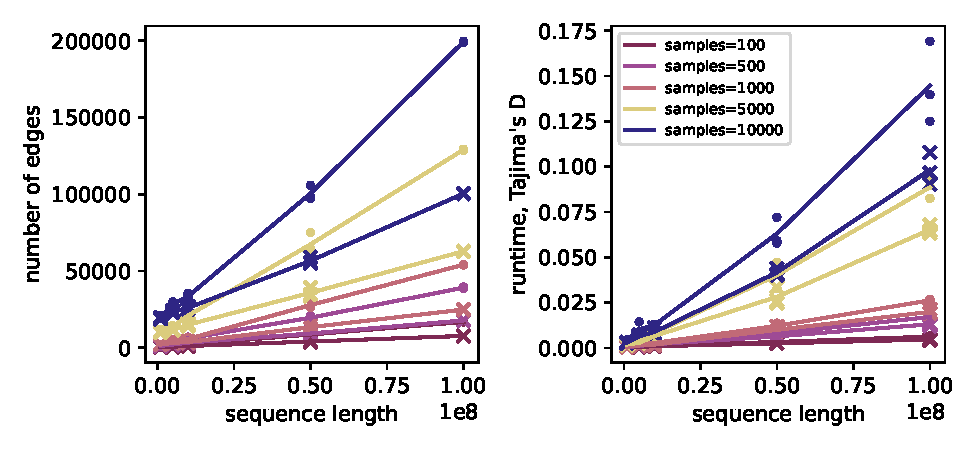
\includegraphics{benchmarks/one_pop_results_absolute_values}
    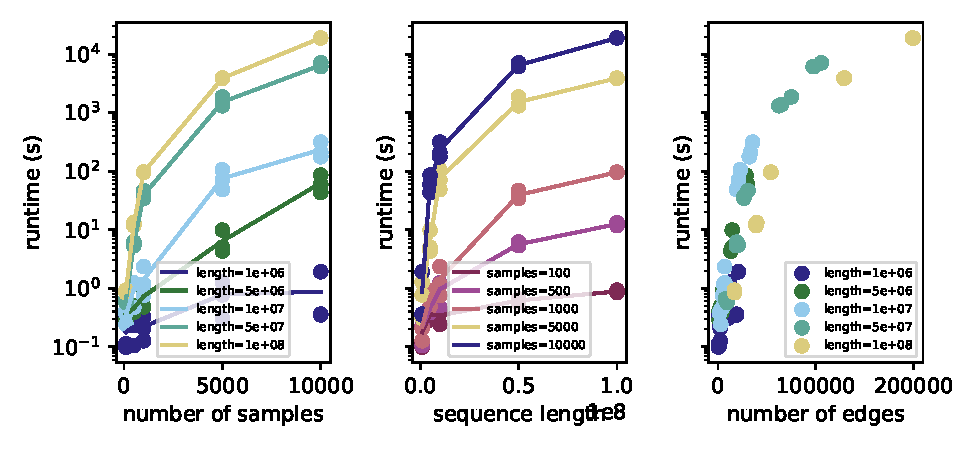
\includegraphics{benchmarks/one_pop_results_timing}
    \caption{
        \textbf{(Above:)}
        Absolute values for ratios shown in \figref{fig:speed_and_edges}:
        \textbf{(left)} numbers of edges; and
        \textbf{(right)} runtime.
        \textbf{(Below:)} runtime for the \texttt{extend\_haplotypes}
        implementation of \algorithmref{alg:extend} provided in the \tskit{} library.
        For other details, see \figref{fig:speed_and_edges}.
        \label{fig:speed_and_edges_other}
    }
\end{figure}

\begin{figure}
    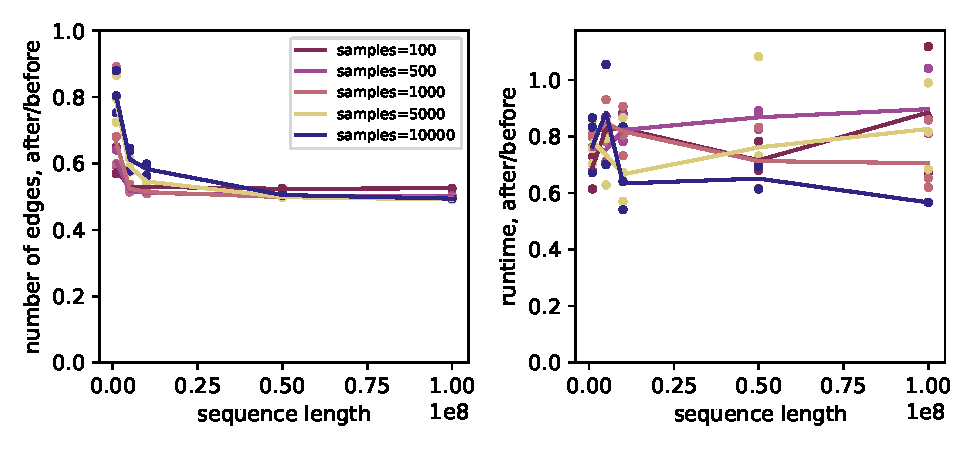
\includegraphics{benchmarks/constant_pop_results_ratios}
    \caption{
        As in \figref{fig:speed_and_edges} except that
        the original tree sequence was simulated with an constant population
        of size $10^4$ (using the ``constant dog'' scenario);
        see Methods for details.
        Absolute values are shown in Supplementary \figref{fig:speed_and_edges_constant_other}.
        \label{fig:speed_and_edges_constant}
    }
\end{figure}

\begin{figure}
    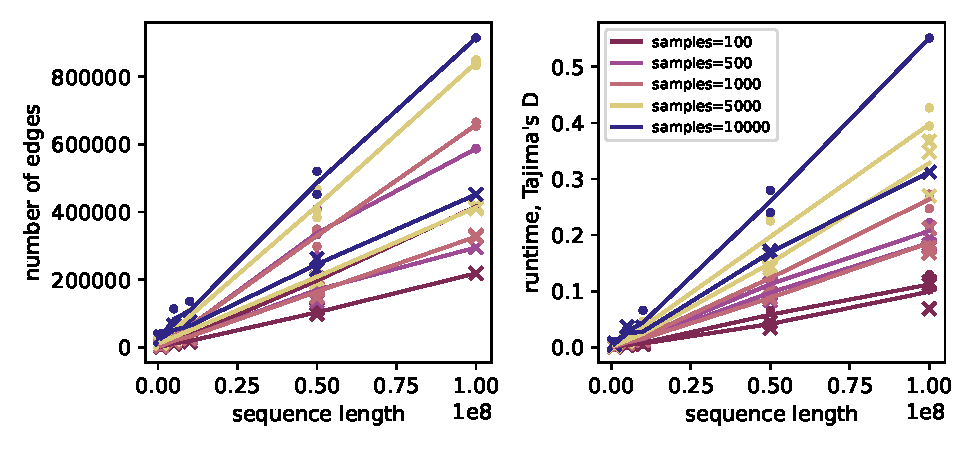
\includegraphics{benchmarks/constant_pop_results_absolute_values}
    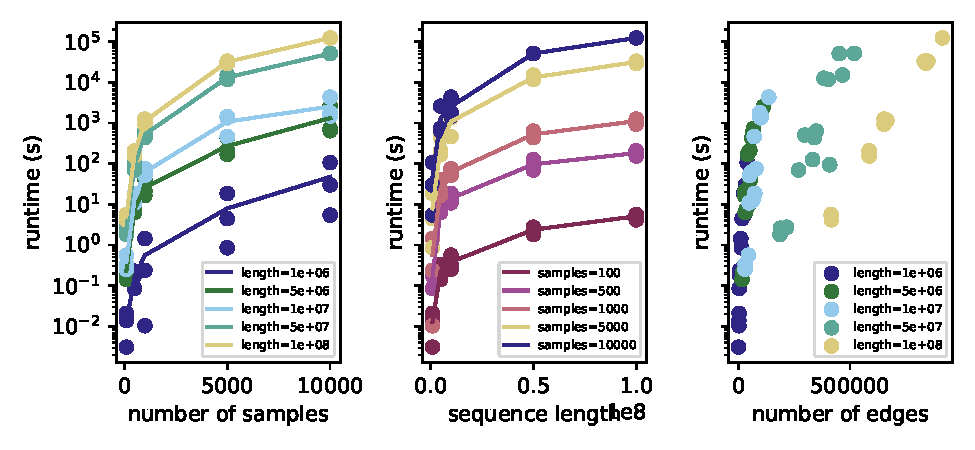
\includegraphics{benchmarks/constant_pop_results_timing}
    \caption{
        As in \figref{fig:speed_and_edges_other} except that
        the original tree sequence was simulated with an constant population
        of size $10^4$ (using the ``constant dog'' scenario).
        \label{fig:speed_and_edges_other_constant}
    }
\end{figure}

\begin{figure}[!hbt]
	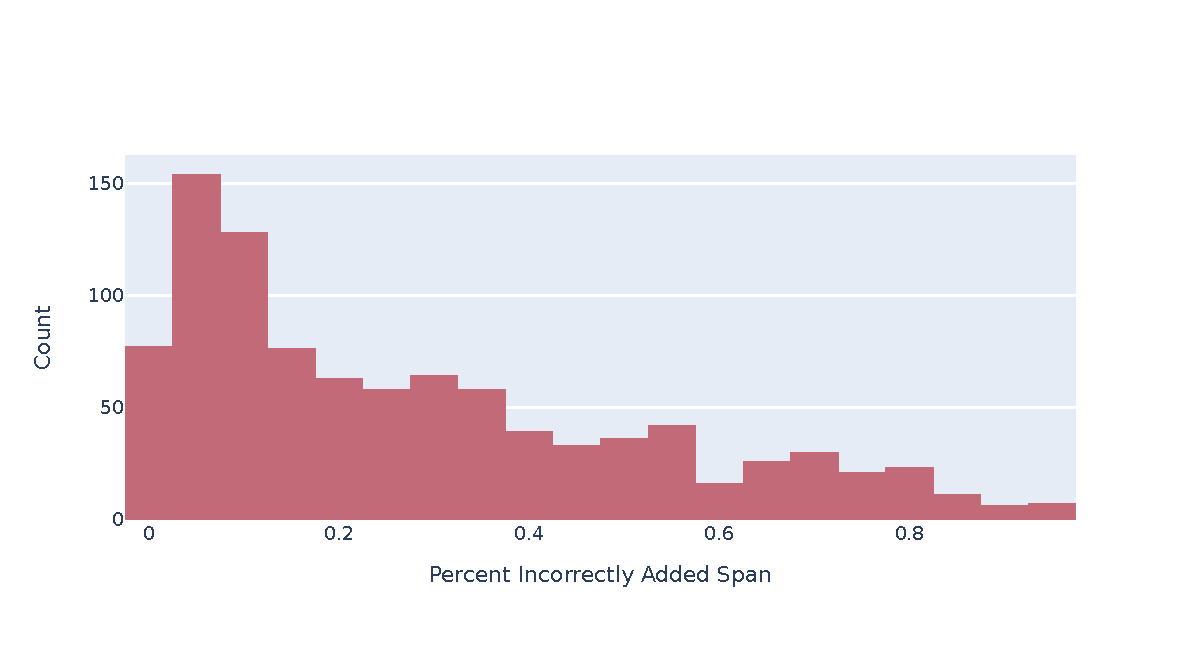
\includegraphics{newplots_wo_ee/figure-4b-supplement}
	\caption{Distribution of incorrectly added span percentages
		for the simulated tree sequence in \figref{fig:node-spans}.}
	\label{fig:incorrect_ratio}
\end{figure}



%\begin{figure}
%    \caption{
%        Supplementary figure: runtime of discrepancy function as a function of number of trees
%        (which we modulate by changing sequence length).
%        \label{fig:speed_discrepancy}
%    }
%\end{figure}


\begin{table}[!hbt]
\begin{center}
\begin{tabular}{|c|c|c|c|c|}
	\hline
	Initial & Iteration 1 & Iteration 2 & Iteration 3 & Iteration 4 \\
	\hline
	\hline
	113463	&	76301	&	76059	&	76057	&	76057 \\
	\hline
	113266 & 76084	&	75835	&	75833	&	75833 \\
	\hline
	114489 & 76703 & 76436 & 76434 & 76434 \\
	\hline
	114086	& 76550	& 76294	& 76291	& 76291\\
	\hline
\end{tabular}
\caption{Number of edges for each iteration of \textit{extend haplotypes} applied to 
simulated tree sequences with sample size $10^4$ and length $5\times 10^7$. 
Each of the simulations terminated by the fourth iteration, however 99\% of the edges
are removed within the first iteration.}
\label{tab:edge-counts}
\end{center}
\end{table}

\end{document}
